%%%%%%%%%%%%  Generated using docx2latex.com  %%%%%%%%%%%%%%

%%%%%%%%%%%%  v2.0.0-beta  %%%%%%%%%%%%%%

\documentclass[12pt]{article}
\usepackage{amsmath}
\usepackage{latexsym}
\usepackage{amsfonts}
\usepackage[normalem]{ulem}
\usepackage{array}
\usepackage{amssymb}
\usepackage{graphicx}
%\usepackage[backend=biber,
%style=numeric,
%sorting=none,
%isbn=false,
%doi=false,
%url=false,
%{biblatex}\addbibresource{bibliography.bib}]

\usepackage{subfig}
\usepackage{wrapfig}
\usepackage{wasysym}
\usepackage{enumitem}
\usepackage{adjustbox}
\usepackage{ragged2e}

\usepackage[svgnames,table]{xcolor}
\usepackage{tikz}
\usepackage{longtable}
\usepackage{changepage}
\usepackage{setspace}
\usepackage{hhline}
\usepackage{multicol}
\usepackage{tabto}
\usepackage{float}
\usepackage{multirow}
\usepackage{makecell}
\usepackage{fancyhdr}
\usepackage[toc,page]{appendix}
\usepackage[hidelinks]{hyperref}
\usetikzlibrary{shapes.symbols,shapes.geometric,shadows,arrows.meta}
\tikzset{>={Latex[width=1.5mm,length=2mm]}}
\usepackage{flowchart}\usepackage[paperheight=11.0in,paperwidth=8.5in,left=1.0in,right=1.0in,top=1.0in,bottom=1.0in,headheight=1in]{geometry}
\usepackage[utf8]{inputenc}
\usepackage[T1]{fontenc}
\TabPositions{0.5in,1.0in,1.5in,2.0in,2.5in,3.0in,3.5in,4.0in,4.5in,5.0in,5.5in,6.0in,}

\urlstyle{same}


 %%%%%%%%%%%%  Set Depths for Sections  %%%%%%%%%%%%%%

% 1) Section
% 1.1) SubSection
% 1.1.1) SubSubSection
% 1.1.1.1) Paragraph
% 1.1.1.1.1) Subparagraph


\setcounter{tocdepth}{5}
\setcounter{secnumdepth}{5}


 %%%%%%%%%%%%  Set Depths for Nested Lists created by \begin{enumerate}  %%%%%%%%%%%%%%


\setlistdepth{9}
\renewlist{enumerate}{enumerate}{9}
		\setlist[enumerate,1]{label=\arabic*)}
		\setlist[enumerate,2]{label=\alph*)}
		\setlist[enumerate,3]{label=(\roman*)}
		\setlist[enumerate,4]{label=(\arabic*)}
		\setlist[enumerate,5]{label=(\Alph*)}
		\setlist[enumerate,6]{label=(\Roman*)}
		\setlist[enumerate,7]{label=\arabic*}
		\setlist[enumerate,8]{label=\alph*}
		\setlist[enumerate,9]{label=\roman*}

\renewlist{itemize}{itemize}{9}
		\setlist[itemize]{label=$\cdot$}
		\setlist[itemize,1]{label=\textbullet}
		\setlist[itemize,2]{label=$\circ$}
		\setlist[itemize,3]{label=$\ast$}
		\setlist[itemize,4]{label=$\dagger$}
		\setlist[itemize,5]{label=$\triangleright$}
		\setlist[itemize,6]{label=$\bigstar$}
		\setlist[itemize,7]{label=$\blacklozenge$}
		\setlist[itemize,8]{label=$\prime$}

\setlength{\topsep}{0pt}\setlength{\parindent}{0pt}

 %%%%%%%%%%%%  This sets linespacing (verticle gap between Lines) Default=1 %%%%%%%%%%%%%%


\renewcommand{\arraystretch}{1.3}


%%%%%%%%%%%%%%%%%%%% Document code starts here %%%%%%%%%%%%%%%%%%%%


\begin{document}
%\begin{Center}
%{\fontsize{36pt}{43.2pt}\selectfont Android 9.0 Pie\par}\par 
%\end{Center}\par

\title{\color{black}COM301T: Operating Systems Assignment 1: \\*Android 9.0 Pie}
\author{{\color{black}COE17B010, COE17B015, COE17B036}}
\date{August 2, 2019}
\maketitle



\setlength{\parskip}{16.08pt}
{
\fontsize{20pt}{22.6pt}\selectfont \textbf{What is an OS?}\par
}\par 
\setlength{\parskip}{8.04pt}
\textcolor[HTML]{4A4A4A}{An OS is a interface between   \textbf{Hardware} and \textbf{End User}.}\par

{\fontsize{20pt}{22.6pt}\selectfont \textbf{Introduction to Android}\par}\par 
\textcolor[HTML]{4A4A4A}{Android is an opensource Operating system based on Linux with a java programming interface for mobile devices such as smartphones as well as tablets.\\*
Android 9.0 Pie is the 9th major release of android (14th overall version) and it has a lot of new features as well as improvements and enhancements over the older versions.}
\par

{\fontsize{18pt}{21.6pt}\selectfont \textbf{\uline{Key Features:}}\par}\par

\setlength{\parskip}{8.04pt}

\textbf{\textcolor[HTML]{4A4A4A}{1. Gesture Based Navigation}}\par

\textcolor[HTML]{4A4A4A}{This is a new feature introduced by Google’s Android wherein you will not be having your home button and recents button instead it is folded into one home screen button so that the users can interact more fluidly.}\par
\textcolor[HTML]{4A4A4A}{The new Android home button reacts somewhat similar to the iPhone X style. Overall, the new gesture navigation feature is very easy to use and doesn’t take long to respond.}\par

\textbf{\textcolor[HTML]{4A4A4A}{2. The Digital Wellbeing Dashboard}}\par

\textcolor[HTML]{4A4A4A}{This feature helps users get more useful insights about how they use phone. For example, it shows how many times you wake up your phone, how much time you spend on various apps, etc. Using this information, a user can now focus on reducing the time he spends while using his phone or an app.and hence optimize his time spent on the smartphone.}\par

\textbf{\textcolor[HTML]{4A4A4A}{3. 'Shush' Feature}}\par

\textcolor[HTML]{4A4A4A}{Shush which is a new gesture will help users easily put their phone to $``$Do Not Disturb$"$  mode by simply flipping their phone screen down. This mode gets automatically enabled when you place your phone screen down.}\par

\textbf{\textcolor[HTML]{4A4A4A}{4. App Actions}}\par

\textcolor[HTML]{4A4A4A}{App actions are actually small actions or commands that trigger a certain app. Since the Android Pie hinges so much on predictability, it also has a feature that pops up the actions when the OS thinks you will need them. For example, the OS will automatically show you the music app popup when you plug in the headphones.}\par

\begin{figure}[t]
\begin{center}
\centering

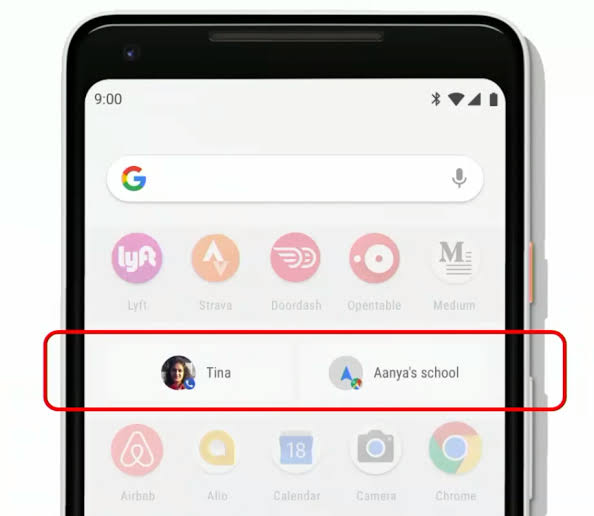
\includegraphics[trim ={0.75cm 0.75cm 0.75cm 0.75cm}, width=0.7\textwidth]{AppAction}\vspace{2mm}
\caption{\textbf{App Actions}: Uses AI to predict next action}
\end{center}
\end{figure}

\textbf{\textcolor[HTML]{4A4A4A}{5. Display Rotation Option}}\par

\textcolor[HTML]{4A4A4A}{The new advanced display rotation feature will probably be the most wildly used feature. If you have the auto rotation feature turned off, every time you rotate your phone the Android Pie will show a rotate icon. The screen will rotate if you click it, else it will disappear after a few seconds.}\par

\textbf{\textcolor[HTML]{4A4A4A}{6. Indoor Positioning with WiFi RTT}}\par
\textcolor[HTML]{4A4A4A}{This feature, with hardware support, apps can now use the RTT (WiFi Round Trip Time) APIs to find distance to nearby RTT capable WiFi access points.}\par

\begin{figure}[ht!]
\begin{center}
\centering

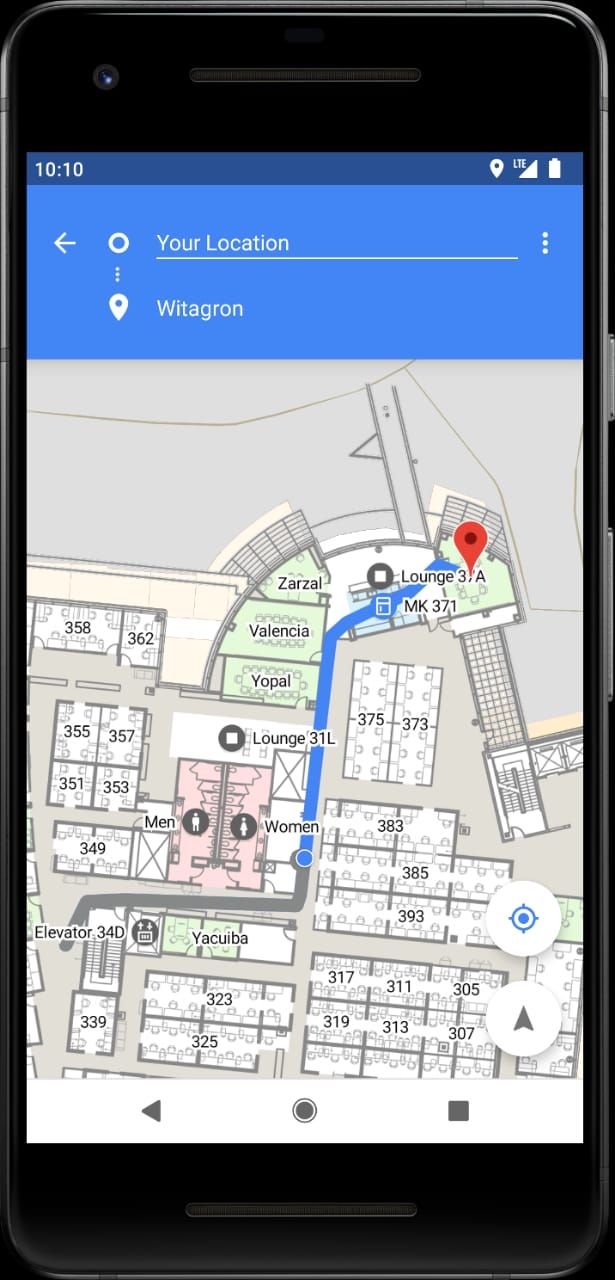
\includegraphics[trim ={1.75cm 10cm 1.75cm 10cm}, clip, width=0.7\textwidth]{RTT}
\caption{\textbf{RTT}: Measures distance to nearest WiFi spots}
\end{center}
\end{figure}

\textbf{\textcolor[HTML]{4A4A4A}{7. It has Dual Camera Support for developers}}\par

\textbf{\textcolor[HTML]{4A4A4A}{8. It offers privacy improvements at apps}}\par

\textbf{\textcolor[HTML]{4A4A4A}{9. It presents new lock options}}\par

\textbf{\textcolor[HTML]{4A4A4A}{10. It has New Emojis}}\par

\textbf{\textcolor[HTML]{4A4A4A}{11. It comes with better indoor navigation and it is easier to take a screenshot}}\par

\textbf{\textcolor[HTML]{4A4A4A}{12. Time display has been moved to top left of screen increasing its visibility}}\par

\textbf{\textcolor[HTML]{4A4A4A}{13. It supports the new notch design in smartphones}}\par

\textbf{\textcolor[HTML]{4A4A4A}{14. It offers improved flow with more speed and more customizations.\\*\\*\\*
}}\par

\setlength{\parskip}{8.04pt}

{\fontsize{18pt}{21.6pt}\selectfont \textbf{\uline{Pros:}}\par}\par

\setlength{\parskip}{8.04pt}

\textbf{\textcolor[HTML]{4A4A4A}{1. Adaptive Battery Utilisation}}\par

\textcolor[HTML]{4A4A4A}{Using the latest AI techniques, the OS will be able to identify and understand which are the apps the user is most likely to use in the next few hours. Using this information, the OS can optimize the smartphone’s CPU usage which can, in turn, improve battery performance by up to 30$\%$ .}\par

\textbf{\textcolor[HTML]{4A4A4A}{2. Adaptive Brightness Adjustments}}\par

\textcolor[HTML]{4A4A4A}{This feature also utilizes AI techniques to adjust the screen brightness according to usage. The screen brightness automatically adjusts to the environment and activities of the user.}\par

\textbf{\textcolor[HTML]{4A4A4A}{3. New Volume $\&$  New Screenshot Interface}}\par

\textcolor[HTML]{4A4A4A}{Concluding\ on the Android Pie's more notable features is a pair of small interface changes like the screenshot and volume UIs. On raising or lowering the volume, Android Pie presents a vertical slider on the right side of the phone, unlike the horizontal element in previous versions. Pressing the volume rocker now modifies media volume by default, instead of the ringer volume.  }\par

\textcolor[HTML]{4A4A4A}{Another noticeable change is the screenshot feature. On taking a screenshot the OS automatically presents options to edit it, where the user can quickly crop or make changes to the picture before saving it.}\par

\textbf{\textcolor[HTML]{4A4A4A}{4. Enhanced Messaging Expierence}}\par

\textcolor[HTML]{4A4A4A}{(i) The user can now send a set of standard responses for messaging which makes it easier for the user because he will not be wasting his time typing the whole message.}\par

\textbf{\textcolor[HTML]{4A4A4A}{5. Enhanced UI}}\par

\textcolor[HTML]{4A4A4A}{(i) In all menu items, notifications etc. all sharp corners have been replaced with round edges giving a better feel.\\*
(ii) All rectangular icons have benn replaced with cirular icons. \\* (iii) Night mode has been added.\\* (iv) Major improvements in Settings App w.r.t UI and classification.}\par


{\fontsize{18pt}{21.6pt}\selectfont \textbf{\uline{Cons:}}\par}\par
\addcontentsline{toc}{subsubsection}{Cons of Android Pie}

\textbf{\textcolor[HTML]{4A4A4A}{1. Gesture Feature}}\par

\textcolor[HTML]{4A4A4A}{As the gesture fetaure is new, it still requires more improvements and time for new users to get used to it. As people have gotten used to separate buttons for home, back and recents, this feature causes a lot of confusion.}\par

\textbf{\textcolor[HTML]{4A4A4A}{2. Notifications}}\par

\textcolor[HTML]{4A4A4A}{Even with enhancements, notifications can be a little overwhelming.
\\*
A lot of features which Google advertised are currently not available. We expect them to be launched soon.}\par

\textbf{\textcolor[HTML]{4A4A4A}{3. Unreleased Features}}\par

\textcolor[HTML]{4A4A4A}{
Many features which were announced are yet to be released.}\par

\textbf{\textcolor[HTML]{4A4A4A}{4. Unsupported Notch}}\par

\textcolor[HTML]{4A4A4A}{
Although all Google apps support the notch design, other apps are yet to adapt to it.}\par

\textbf{\textcolor[HTML]{4A4A4A}{5. Hardware limits}}\par

\textcolor[HTML]{4A4A4A}{
Due to hardware limits, some phones after upgrading start to face performance issues. Also, Android Pie takes up larger space than other versions and hence requires more internal storage.}\par

\textbf{\textcolor[HTML]{4A4A4A}{6. Non-Effective New Features}}\par

\textcolor[HTML]{4A4A4A}{
Even though there are a lot of new features, many of them requires users to adapt to them or needs to be further improved. Eg. Many users are complaining that the shush feature is not reliable.}\par

\par

{\fontsize{20pt}{22.6pt}\selectfont \textbf{Summary}\par}\par 
\textcolor[HTML]{4A4A4A}{Android 9.0 Pie has introduced a lot of really cool and intelligent features that has produced a collection of tools, utilizing machine learning and AI, to provide a lot of comfort and usability. Even though some of its features needs more improvement and may require getting used to, still it cannot be denied that its features like adaptive battery usage and UI enhancements greatly outweigh those cons.}
\par

\vspace{\baselineskip}

%\printbibliography
\end{document}
